%===============================================================================
% LaTeX sjabloon voor de bachelorproef toegepaste informatica aan HOGENT
% Meer info op https://github.com/HoGentTIN/latex-hogent-report
%===============================================================================

\documentclass[dutch,dit,thesis]{hogentreport}

% TODO:
% - If necessary, replace the option `dit`' with your own department!
%   Valid entries are dbo, dbt, dgz, dit, dlo, dog, dsa, soa
% - If you write your thesis in English (remark: only possible after getting
%   explicit approval!), remove the option "dutch," or replace with "english".

\usepackage{lipsum} % For blind text, can be removed after adding actual content

%% Pictures to include in the text can be put in the graphics/ folder
\graphicspath{{graphics/}}

%% For source code highlighting, requires pygments to be installed
%% Compile with the -shell-escape flag!
%% \usepackage[section]{minted}
%% If you compile with the make_thesis.{bat,sh} script, use the following
%% import instead:
\usepackage[section,outputdir=../output]{minted}
\usemintedstyle{solarized-light}
\definecolor{bg}{RGB}{253,246,227} %% Set the background color of the codeframe

%% Change this line to edit the line numbering style:
\renewcommand{\theFancyVerbLine}{\ttfamily\scriptsize\arabic{FancyVerbLine}}

%% Macro definition to load external java source files with \javacode{filename}:
\newmintedfile[javacode]{java}{
    bgcolor=bg,
    fontfamily=tt,
    linenos=true,
    numberblanklines=true,
    numbersep=5pt,
    gobble=0,
    framesep=2mm,
    funcnamehighlighting=true,
    tabsize=4,
    obeytabs=false,
    breaklines=true,
    mathescape=false
    samepage=false,
    showspaces=false,
    showtabs =false,
    texcl=false,
}

% Other packages not already included can be imported here

%%---------- Document metadata -------------------------------------------------
% TODO: Replace this with your own information
\author{Quinten De Wolf}
\supervisor{Mevr M. Van Audenrode}
\cosupervisor{Mr. D. Van Der Elst}
\title[Optionele ondertitel]%
    {Titel van de bachelorproef}
\academicyear{\advance\year by -1 \the\year--\advance\year by 1 \the\year}
\examperiod{1}
\degreesought{\IfLanguageName{dutch}{Professionele bachelor in de toegepaste informatica}{Bachelor of applied computer science}}
\partialthesis{false} %% To display 'in partial fulfilment'
%\institution{Internshipcompany BVBA.}

%% Add global exceptions to the hyphenation here
\hyphenation{back-slash}

%% The bibliography (style and settings are  found in hogentthesis.cls)
\addbibresource{bachproef.bib}            %% Bibliography file
\addbibresource{../voorstel/voorstel.bib} %% Bibliography research proposal
\defbibheading{bibempty}{}

%% Prevent empty pages for right-handed chapter starts in twoside mode
\renewcommand{\cleardoublepage}{\clearpage}

\renewcommand{\arraystretch}{1.2}

%% Content starts here.
\begin{document}

%---------- Front matter -------------------------------------------------------

\frontmatter

\hypersetup{pageanchor=false} %% Disable page numbering references
%% Render a Dutch outer title page if the main language is English
\IfLanguageName{english}{%
    %% If necessary, information can be changed here
    \degreesought{Professionele Bachelor toegepaste informatica}%
    \begin{otherlanguage}{dutch}%
       \maketitle%
    \end{otherlanguage}%
}{}

%% Generates title page content
\maketitle
\hypersetup{pageanchor=true}

%%=============================================================================
%% Voorwoord
%%=============================================================================

\chapter*{\IfLanguageName{dutch}{Woord vooraf}{Preface}}%
\label{ch:voorwoord}

%% TODO:
%% Het voorwoord is het enige deel van de bachelorproef waar je vanuit je
%% eigen standpunt (``ik-vorm'') mag schrijven. Je kan hier bv. motiveren
%% waarom jij het onderwerp wil bespreken.
%% Vergeet ook niet te bedanken wie je geholpen/gesteund/... heeft

Met trots presenteer ik mijn bachelorproef "De beste JavaScript runtime-omgeving voor performante applicaties: een vergelijkende studie", 
waarin ik, in het kader voor het voltooien van mijn opleiding Toegepaste Informatica, Node.js vergelijk met het opkomende Bun op vlak van performantie.
Tijdens mijn studiejaren ben ik altijd geïnteresseerd geweest in JavaScript runtime-omgevingen zoals onder andere Node.js en Bun en
hoe deze tegen over elkaar staan. Toen ik een onderwerp moest kiezen kwam dit direct in me op aangezien het mij interessant leek om me dieper te verdiepen 
in Bun. Het schrijven van deze bachelorproef heeft me dan ook uitgedaagd om mijn kennis en vaardigheden te verbreden.
\vspace{5mm}
Ik wil mijn oprechte dank betuigen aan iedereen die heeft bijgedragen aan deze bachelorproef, 
in het bijzonder mijn promotor Mevr M. Van Audenrode en mijn co-promotor Mr. D. Van Der Elst voor hun
waardevolle begeleiding en feedback gedurende het hele proces. 
Zij stonden altijd klaar voor vragen en gaven telkens constructieve en gerichte feedback waarvoor ik hun zeer dankbaar ben.
\vspace{5mm}

Tot slot wil ik mijn ouders bedanken voor de kansen die zij mij hebben gegeven. 
Dankzij hun dagelijkse inzet kan ik mij telkens concentreren op mijn studies.



%%=============================================================================
%% Samenvatting
%%=============================================================================

% TODO: De "abstract" of samenvatting is een kernachtige (~ 1 blz. voor een
% thesis) synthese van het document.
%
% Een goede abstract biedt een kernachtig antwoord op volgende vragen:
%
% 1. Waarover gaat de bachelorproef?
% 2. Waarom heb je er over geschreven?
% 3. Hoe heb je het onderzoek uitgevoerd?
% 4. Wat waren de resultaten? Wat blijkt uit je onderzoek?
% 5. Wat betekenen je resultaten? Wat is de relevantie voor het werkveld?
%
% Daarom bestaat een abstract uit volgende componenten:
%
% - inleiding + kaderen thema
% - probleemstelling
% - (centrale) onderzoeksvraag
% - onderzoeksdoelstelling
% - methodologie
% - resultaten (beperk tot de belangrijkste, relevant voor de onderzoeksvraag)
% - conclusies, aanbevelingen, beperkingen
%
% LET OP! Een samenvatting is GEEN voorwoord!

%%---------- Nederlandse samenvatting -----------------------------------------
%
% TODO: Als je je bachelorproef in het Engels schrijft, moet je eerst een
% Nederlandse samenvatting invoegen. Haal daarvoor onderstaande code uit
% commentaar.
% Wie zijn bachelorproef in het Nederlands schrijft, kan dit negeren, de inhoud
% wordt niet in het document ingevoegd.

\IfLanguageName{english}{%
\selectlanguage{dutch}
\chapter*{Samenvatting}
\lipsum[1-4]
\selectlanguage{english}
}{}

%%---------- Samenvatting -----------------------------------------------------
% De samenvatting in de hoofdtaal van het document

\chapter*{\IfLanguageName{dutch}{Samenvatting}{Abstract}}

Performantie is doorheen de tijd alsmaar belangrijker geworden. 
Een goed presterende applicatie draagt bij aan een betere gebruikerservaring.
Gedurende deze tijd zijn er voortdurend nieuwe JavaScript runtime-omgevingen ontwikkeld met telkens nieuwe verbeteringen om
zo de noden van de alsmaar complexere applicaties te vervullen. 
Ondanks deze nieuwe ontwikkelingen worden weinig ervan effectief in de praktijk gebruikt.
Zo wordt het oudere Node.js vaak nog gekozen als JavaScript runtime-omgeving bij de ontwikkeling van applicaties.
Dit onderzoek heeft als doel inzicht te verschaffen in de performantie van Node.js en één van deze nieuwe omgevingen
om zo een correcte keuze te kunnen maken bij de ontwikkeling van performante applicaties.
De onderzoeksvraag hierbij is of één van deze nieuwe frameworks  
een correcte plaatsvervanger kan zijn voor Node.js bij de ontwikkeling van applicaties binnen bedrijven 
waar performantie centraal staat. Het onderzoek kan dan gebruikt worden als basis 
voor het maken van een doordachte backend keuze.
Om een antwoord te bekomen werd eerst informatie over het onderzoeksdomein verzameld om zo een duidelijk beeld ervan te schetsen.
Hierbij werden in de literatuurstudie Javascript runtime-omgevingen zoals Node.js, Deno en Bun besproken.
Nadien wordt aan de hand van een requirements-analyse één omgeving geselecteerd die het meest geschikt is als potentiële plaatsvervanger voor Node.js.
Hierbij voldeed Bun aan alle requirements en werd er gekozen om deze omgeving te vergelijken met Node.js in de proof-of-concepts.
Aan de hand van het Quick Sort algoritme werd de performantie bij computationele berekeningen gemeten.
Daarnaast werd ook een applicatie opgesteld met de mogelijkheid om data op te halen en in te voegen. 
Hierbij werd de performantie van beide omgevingen gemeten bij het afhandelen van netwerkverzoeken.
Dezelfde applicatie werd ook gebruikt om de installatietijd van de respectievelijke package managers te meten.
Hierbij heeft Bun een snellere installatietijd dan Node.js.
Bij het meten van het Quick Sort algoritme heeft Bun ook een snellere uitvoeringstijd wat het standpunt 
ondersteunt dat Bun beter presteert bij het uitvoeren van computationele berekeningen.
Tot slot heeft Bun een lagere latentie en een betere verwerking van het aantal verzoeken per seconde bij het ophalen en
invoegen van data ten koste van het CPU-gebruik en geheugengebruik.
Dit leidt tot de conclusie dat Bun een optimale keuze kan zijn voor applicaties met complexe algoritmes en calculaties. Echter, 
bij applicaties waarbij I/O-taken worden uitgevoerd, moet telkens een afweging gemaakt worden tussen de snellere verwerking van Bun
en het hogere middelengebruik dathiermee gepaard gaat.




%---------- Inhoud, lijst figuren, ... -----------------------------------------

\tableofcontents

% In a list of figures, the complete caption will be included. To prevent this,
% ALWAYS add a short description in the caption!
%
%  \caption[short description]{elaborate description}
%
% If you do, only the short description will be used in the list of figures

\listoffigures

% If you included tables and/or source code listings, uncomment the appropriate
% lines.
%\listoftables
\listoflistings

% Als je een lijst van afkortingen of termen wil toevoegen, dan hoort die
% hier thuis. Gebruik bijvoorbeeld de ``glossaries'' package.
% https://www.overleaf.com/learn/latex/Glossaries

%---------- Kern ---------------------------------------------------------------

\mainmatter{}

% De eerste hoofdstukken van een bachelorproef zijn meestal een inleiding op
% het onderwerp, literatuurstudie en verantwoording methodologie.
% Aarzel niet om een meer beschrijvende titel aan deze hoofdstukken te geven of
% om bijvoorbeeld de inleiding en/of stand van zaken over meerdere hoofdstukken
% te verspreiden!

%%=============================================================================
%% Inleiding
%%=============================================================================

\chapter{\IfLanguageName{dutch}{Inleiding}{Introduction}}%
\label{ch:inleiding}


Door de jaren heen zijn applicaties alsmaar complexer geworden. Hierbij worden vaak achterliggend netwerkverzoeken afgehandeld door een 
een backend applicatie. Deze applicatie draait in een runtime-omgeving buiten de browser, 
waardoor deze toegang heeft tot databanken en netwerken van de server waarop het wordt uitgevoerd.
Een manier om zo een backend te ontwikkelen is met behulp van de programmeertaal JavaScript. 
Backend JavaScript applicaties worden dan uitgevoerd in een JavaScript runtime omgeving.
De meest populaire omgeving is Node.js. Zo toont onderzoek van ~\textcite{Greif2022} aan dat 93.6\% van de 29888 bevraagden Node.js 
regulier gebruiken.
Dit tegenover de 11.2\% en 4.3\% van de mensen die andere omgevingen zoals respectievelijk Deno en Bun gebruiken.
Deze 2 omgevingen zijn relatief jonger dan Node.js.

\section{\IfLanguageName{dutch}{Probleemstelling}{Problem Statement}}%
\label{sec:probleemstelling}

Performantie is doorheen de tijd alsmaar belangrijker geworden. 
Een performante applicatie zorgt hierbij voor een betere gebruikerservaring. 
Momenteel blijft Node.js de standaard keuze voor veel projecten. Niettemin zijn er nog tal van andere JavaScript runtime-omgevingen
, zoals Bun en Deno, die in staat zijn om de specifieke noden te vervullen waar Node.js niet aan kan voldoen. In dit onderzoek wordt geprobeerd 
een inzicht te verschaffen in de performantie van Node.js en één van deze nieuwe omgevingen,
om zo een weloverwogen keuze te kunnen maken bij de ontwikkeling van performante applicaties.
Dit onderzoek is relevant voor bedrijven waar performantie een essentiële rol speelt binnen de ontwikkeling van JavaScript backend applicaties en kan dienen als basis 
voor het maken van een doordachte backend keuze. Dit onderzoek 
biedt ook inzicht in de capaciteiten van Bun voor andere betrokkenen binnen het vakgebied van JavaScript backend ontwikkeling.

\section{\IfLanguageName{dutch}{Onderzoeksvraag}{Research question}}%
\label{sec:onderzoeksvraag}

In dit onderzoek wordt bestudeerd of één van deze nieuwe omgevingen
een correcte plaatsvervanger kan zijn voor Node.js bij de ontwikkeling van performante applicaties binnen bedrijven 
waar een JavaScript runtime wordt gebruikt.
Hierbij spelen verschillende aspecten een rol die aan de hand van volgende deelvragen worden onderzocht:
\begin{itemize}
  \item Wat zijn de onderliggende verschillen tussen Node.js en de andere omgeving?
  \item Is de gekozen omgeving performanter dan Node.js bij het uitvoeren van computationele berekeningen?
  \item Is de gekozen omgeving performanter dan Node.js bij het afhandelen van netwerkverzoeken?
  \item Wat is het verschil tussen hun respectievelijke package managers?
\end{itemize}

\section{\IfLanguageName{dutch}{Onderzoeksdoelstelling}{Research objective}}%
\label{sec:onderzoeksdoelstelling}

Dit onderzoek heeft als doel inzicht te verschaffen in de performantie van Node.js en één van deze nieuwe omgevingen
om zo een correcte keuze te kunnen maken bij de ontwikkeling van performante applicaties. Dit wordt bereikt door middel van een vergelijkende studie
waarbij zowel de geselecteerde omgeving als Node.js worden getest aan de hand proof-of-concepts. 
Hierbij worden de prestaties gemeten tijdens computationele berekeningen en het afhandelen van netwerkverzoeken, waarbij specifiek gekeken wordt naar
de latentie, aantal verzoeken per seconde, installatietijd en uitvoeringstijd. 
Het doel is deze resultaten te gebruiken om vast te stellen of de gekozen omgeving performanter is dan Node.js. 
Het onderzoek wordt als succesvol beschouwd als er aan de hand van deze resultaten een duidelijk verschil tussen de omgevingen zichtbaar is.
\section{\IfLanguageName{dutch}{Opzet van deze bachelorproef}{Structure of this bachelor thesis}}%
\label{sec:opzet-bachelorproef}

% Het is gebruikelijk aan het einde van de inleiding een overzicht te
% geven van de opbouw van de rest van de tekst. Deze sectie bevat al een aanzet
% die je kan aanvullen/aanpassen in functie van je eigen tekst.

De rest van deze bachelorproef is als volgt opgebouwd:

In hoofdstuk~\ref{ch:stand-van-zaken} wordt een overzicht gegeven van de stand van zaken binnen het onderzoeksdomein,
 op basis van een literatuurstudie.

In hoofdstuk~\ref{ch:methodologie} wordt de methodologie toegelicht en worden de gebruikte onderzoekstechnieken besproken om een antwoord te kunnen formuleren 
op de onderzoeksvragen.

In hoofdstuk~\ref{ch:selectie} wordt de lijst van omgevingen afgetoetst aan de opgegegeven requirements om uiteindelijk een geschikte omgeving te selecteren.

In hoofdstuk~\ref{ch:proof-of-concept} wordt de opzet en metingen van de proof-of-concepts toegelicht. Op het einde worden de bekomen resultaten besproken.

In hoofdstuk~\ref{ch:conclusie}, tenslotte, 
wordt de conclusie gegeven en een antwoord geformuleerd op de onderzoeksvragen. 
Daarbij wordt ook een aanzet gegeven voor toekomstig onderzoek binnen dit domein.
\chapter{\IfLanguageName{dutch}{Stand van zaken}{State of the art}}%
\label{ch:stand-van-zaken}

% Tip: Begin elk hoofdstuk met een paragraaf inleiding die beschrijft hoe
% dit hoofdstuk past binnen het geheel van de bachelorproef. Geef in het
% bijzonder aan wat de link is met het vorige en volgende hoofdstuk.

% Pas na deze inleidende paragraaf komt de eerste sectiehoofding.

Dit hoofdstuk bevat je literatuurstudie. 
De inhoud gaat verder op de inleiding, maar zal het onderwerp van de bachelorproef *diepgaand* uitspitten. 
De bedoeling is dat de lezer na lezing van dit hoofdstuk helemaal op de hoogte is van de huidige stand van zaken (state-of-the-art) 
in het onderzoeksdomein. 
Iemand die niet vertrouwd is met het onderwerp, 
weet nu voldoende om de rest van het verhaal te kunnen volgen, 
zonder dat die er nog andere informatie moet over opzoeken \autocite{Pollefliet2011}.

Je verwijst bij elke bewering die je doet, vakterm die je introduceert, enz.\ naar je bronnen. 
In \LaTeX{} kan dat met het commando \texttt{$\backslash${textcite\{\}}} of \texttt{$\backslash${autocite\{\}}}. 
Als argument van het commando geef je de ``sleutel'' van een ``record'' in een bibliografische databank in het Bib\LaTeX{}-formaat
 (een tekstbestand). Als je expliciet naar de auteur verwijst in de zin (narratieve referentie), 
 gebruik je \texttt{$\backslash${}textcite\{\}}. Soms is de auteursnaam niet expliciet een onderdeel van de zin, 
 dan gebruik je \texttt{$\backslash${}autocite\{\}} (referentie tussen haakjes). Dit gebruik je bv.~bij een citaat, 
 of om in het bijschrift van een overgenomen afbeelding, broncode, tabel, enz. te verwijzen naar de bron. 
 In de volgende paragraaf een voorbeeld van elk.

\textcite{Knuth1998} schreef een van de standaardwerken over sorteer- en zoekalgoritmen. 
Experten zijn het erover eens dat cloud computing een interessante opportuniteit vormen, zowel voor gebruikers als voor dienstverleners op vlak van informatietechnologie~\autocite{Creeger2009}.

Let er ook op: het \texttt{cite}-commando voor de punt, dus binnen de zin. Je verwijst meteen naar een bron in de eerste zin die erop gebaseerd is, 
dus niet pas op het einde van een paragraaf.



Dit hoofdstuk bevat een literatuurstudie die de gebruikten technologieën gaat omschrijven. 
Daarnaast worden ook eerdere studies naar deze technologieën vermeld. 
Ten eerste wordt een precieze beschrijving gegeven over de programmeertaal javascript en hoe deze wordt gebruikt bij de runtime-omgevingen.
Nadien wordt verder ingegaan op 2 van deze omgevingen namelijk Node.js en Bun.

\section{Javascript}
Javascript is een programmeertaal die gebruikt wordt om applicaties te ontwikkelen. 
Specifiek is het een scripting taal die gebruikt om web pagina's interactief te maken~\autocite{Mozilla2023}.
Hierbij spreken we over client-side Javascript. Wanneer een web pagina wordt bekeken zal de javascript code worden 
gedownload en uitgevoerd~\autocite{JonathanBrownCFA2024}. Langs de andere kant heb je ook nog Server-side javascript. 
Hierbij wordt de code uitgevoerd op de server in plaats van op de client~\autocite{JonathanBrownCFA2024}. 
Voor deze code dan te laten uitvoeren is een javascript runtime-omgeving nodig. 

\subsection{Javascript runtime-omgeving}
Een javascript-omgeving bestaat uit alle componenten om javascript correct te laten werken ~\autocite{Christopher}. 
Het bevat een JavaScript engine, WEB APIs en een callback queue ~\autocite{Christopher}. 
Deze runtime zal dan javascript code omzetten in code die verstaanbaar is voor de computer.
De omgeving specificeert waar dit wordt gedaan, dit kan in een browser maar ook in andere omgevingen zoals een server.
Met behulp van javascript runtime-omgevingen zoals Node.js en Bun kan javascript code ook buiten de browser worden uitgevoerd~\autocite{Mozilla2023}.

\subsubsection{Javascript engine, WEB APIs en callback queue}

In een artikel van ~\textcite{Christopher}, 
wordt uitgelegd dat de javascript engine een simpel computer programma is dat de code kan interpreteren en uitvoeren.
Elk browser heeft zijn eigen Javascript engine achterliggend. Het meest bekende hiervan is de
V8 engine die zowel bij Google chrome als Node.js wordt gebruikt. 
Wanneer een stuk code in de engine wordt gestoken zal deze eerst gelezen worden (parsing). 
De code wordt hierbij omgezet in een data structuur genaamd abstract syntax tree (AST).
Wanneer deze boom is aangemaakt zal de compiler deze omzetten naar machine code. 
Eenmaal deze code is gegenereerd zal de engine zogenaamde execution contexts aanmaken om de code uit te voeren.
In figuur ~\ref{fig:javascriptengine} wordt hiervan een visuele voorstelling getoond.
\begin{figure}[H]
    \centering
    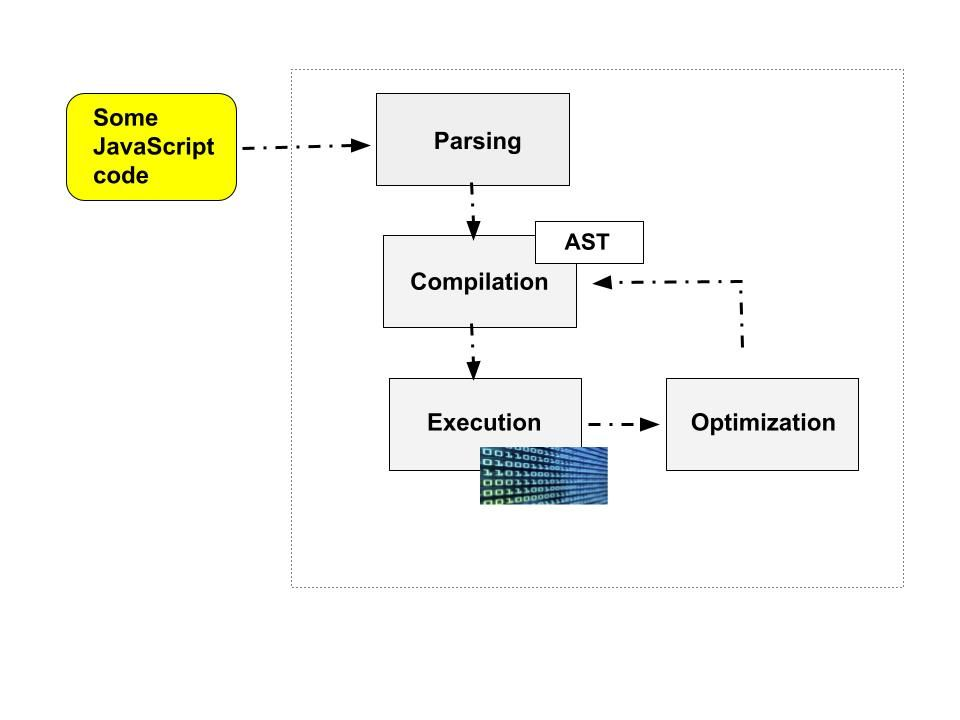
\includegraphics[width=.9\textwidth]{graphics/javascriptengine.jpeg}
    \caption{\label{fig:javascriptengine}}Visuele voorstelling van werking javascript engine ~\autocite{Christopher}.
\end{figure}

Naast een Javascript engine bevat een runtime-omgeving ook WEB APIs en een callback queue. 
WEB APIs zijn functionaliteiten die specifiek voor de runtime omgeving zijn en dus geen deel uitmaken van de javascript taal.
De callback queue zorgt ervoor dat callback functions volgens de First-In-First-Out methode worden uitgevoerd.

\section{Node.js}
De afgelopen jaren is het aantal runtime-omgevingen sterk toegenomen. De meest bekende en oudste hiervan is Node.js.
Node.js is een server-side framework dat wordt gebruikt voor schaalbare applicaties te maken ~\autocite{Gackenheimer2013}.
Het maakt gebruik van de javascript V8 engine ontwikkeld door Google en heeft zijn eigen package manager genaamd Node Package Manager (npm).

\subsection{Event loop}
In het boek van ~\textcite{Ali2013} wordt verteld hoe Node.js zich onderscheidt van andere platformen door het gebruik van een event loop.
Wanneer in Node.js data wordt gelezen of geschreven zal een gebeurtenis worden uitgezonden. 
Aan de hand van zelfgedefinieerde callbacks, verwijzingen naar uitvoerbare code, kan gereageerd worden op deze gebeurtenissen. 
De event loop zal hierbij continu kijken of er gebeurtenissen voorkomen, en wanneer dit zo is zal het deze in de event wachtrij plaatsen.
De event loop zal dan deze wachtrij doorgaan en één per één de event handlers uitvoeren. 
Dit laat toe om I/O operaties asynchroon te maken zonder hierbij multithreading te gebruiken.
In figuur ~\ref{fig:eventloop} wordt hiervan een visuele voorstelling getoond.
\begin{figure}[h]
    \centering
    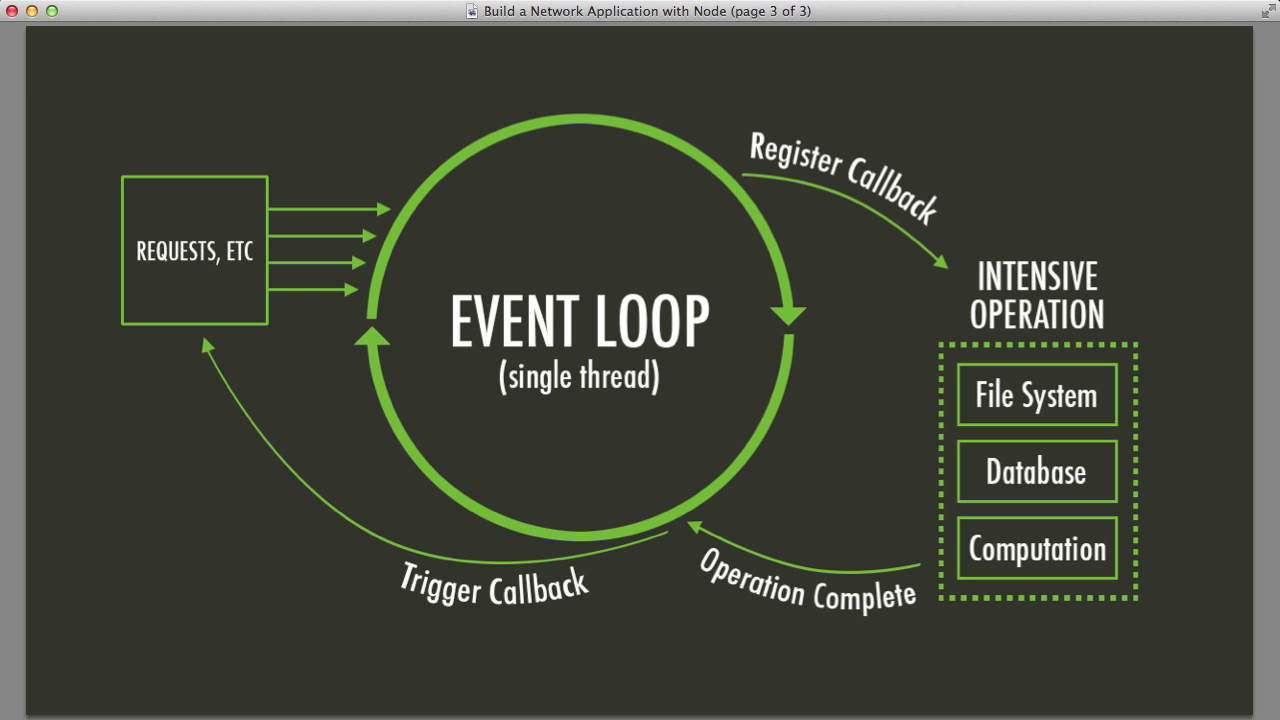
\includegraphics[width=.9\textwidth]{graphics/eventloop.png}
    \caption{\label{fig:eventloop}}Visuele voorstelling van de event loop ~\autocite{Luxembourg2023}.
\end{figure}

\subsection{Node Package Manager}
Node.js maakt gebruik van modules om code te hergebruiken. 
Zo vormt een module een stuk herbruikbare javascript code 
die je kan importeren in een ander javascript bestand ~\autocite{Semah2022}.
Naast deze zelf te maken kan je ook modules of packages van andere ontwikkelaars gebruiken met behulp van de Node Package Manager.
Veel van deze packages hangen af van nog andere packages om correct te werken \autocite{kula2017}.
Aan de hand van een package.json bestand kunnen packages toegevoegd worden aan een project.
\begin{figure}[h!]
    \centering
    \begin{minted}[bgcolor=bg,
        fontfamily=tt,
        linenos=true,
        numberblanklines=true,
        numbersep=5pt,
        gobble=0,
        framesep=2mm,
        tabsize=4,
        obeytabs=false,
        breaklines=true,
        mathescape=false
        samepage=false,
        showspaces=false,
        showtabs =false,
        texcl=false]{js}
        {
          "dependencies": {
            "foo": "1.0.0 - 2.9999.9999",
            "bar": ">=1.0.2 <2.1.2",
            "baz": ">1.0.2 <=2.3.4",
            "boo": "2.0.1",
            "qux": "<1.0.0 || >=2.3.1 <2.4.5 || >=2.5.2 <3.0.0",
            "asd": "http://asdf.com/asdf.tar.gz",
            "til": "~1.2",
            "elf": "~1.2.3",
            "two": "2.x",
            "thr": "3.3.x",
            "lat": "latest",
            "dyl": "file:../dyl"
            }
        }
        \end{minted}
        \caption{Voorbeeld package.json \autocite{Kaplan2024}}
\end{figure}

\section{Bun}
Performantie is één van de belangrijkste zaken bij een server-side framework. 
Daarom is Node.js dankzij zijn event-gedreven I/O model een veelvoorkomende keuze als het gaat om server-side frameworks.
Echter wil Bun dit veranderen door nog meer focus te leggen op snelheid en performantie.

\subsection{JavascriptCore}
Eén van de manieren waardoor Bun dit bereikt is door het gebruiken van een andere Javascript engine.
Bun gebruikt JavaScriptCore in plaats van de V8 Javascript engine die Node.js gebruikt. 
Deze zou volgens ~\textcite{McDonnel2023} ervoor zorgen dat Bun 4 keer sneller opstart dan Node.js. 
De engine is ingebouwd in WebKit, een web browser engine die wordt gebruikt binnen het Apple ecosysteem voor macOS en IOS.
In een artikel van ~\textcite{Pizlo2020} wordt uitgelegd dat bij de executie een script door verschillende fases gaat:
\begin{itemize}
    \item De lexer is verantwoordelijking voor het opbreken van het script in een reeks tokens.
    \item De parser gaat deze tokens gebruiken om een een asbract syntax tree te maken.
    \item De Low-Level Interpreter (LLINT) zal bytecode produceren dat JavaScriptCore kan uitvoeren.
\end{itemize}
Daarnaast zijn er hierbij ook nog optimalisaties voor instructies die vaak terugkeren. 
JavascriptCore zal instructies in 4 verschillende lagen uitvoeren, afhankelijk van hoeveel keer ze worden uitgevoerd:
\begin{enumerate}
    \item De Low-Level Interpreter (LLINT) zal zoals hierboven beschreven instructies omzetten in bytecode.
    \item De baseline JIT zal een stuk code at runtime uitvoeren in plaats van ervoor. 
    Hierbij worden de bytecode operaties omgezet naar een template van machine code zonder veel optimalisaties. Deze laag is snel.
    \item De Data Flow Graph JIT zal een data-flow graaf gebruiken van de code om zo complexe optimalisaties uit te voeren die betrekking hebben tot de stroom van de code.
    \item De Faster than Light JIT zal nog meer optimalisaties toevoegen bovenop de optimalisaties van de Data Flowh Graph JIT. 
    Deze laag is duurder en wordt enkel gebruikt voor code die kunnen profiteren van optimalisaties.
\end{enumerate}
Via de Low-Level Interpreter zal een profile voor elke instructie aangemaakt worden. 
Aan de hand hiervan weet de engine hoeveel keer een instructie wordt uitgevoerd en in welk niveau ze zitten.
LLINT zorgt ervoor dat het geheugengebruik wordt gereduceerd. Zo kost het genereren van machine code zeer veel geheugen.
Doormiddel van LLINT moeten we niet voor alle javascript code de bijhorende machine code genereren.
%%=============================================================================
%% Methodologie
%%=============================================================================

\chapter{\IfLanguageName{dutch}{Methodologie}{Methodology}}%
\label{ch:methodologie}

%% TODO: In dit hoofstuk geef je een korte toelichting over hoe je te werk bent
%% gegaan. Verdeel je onderzoek in grote fasen, en licht in elke fase toe wat
%% de doelstelling was, welke deliverables daar uit gekomen zijn, en welke
%% onderzoeksmethoden je daarbij toegepast hebt. Verantwoord waarom je
%% op deze manier te werk gegaan bent.
%% 
%% Voorbeelden van zulke fasen zijn: literatuurstudie, opstellen van een
%% requirements-analyse, opstellen long-list (bij vergelijkende studie),
%% selectie van geschikte tools (bij vergelijkende studie, "short-list"),
%% opzetten testopstelling/PoC, uitvoeren testen en verzamelen
%% van resultaten, analyse van resultaten, ...
%%
%% !!!!! LET OP !!!!!
%%
%% Het is uitdrukkelijk NIET de bedoeling dat je het grootste deel van de corpus
%% van je bachelorproef in dit hoofstuk verwerkt! Dit hoofdstuk is eerder een
%% kort overzicht van je plan van aanpak.
%%
%% Maak voor elke fase (behalve het literatuuronderzoek) een NIEUW HOOFDSTUK aan
%% en geef het een gepaste titel.

Het onderzoek bevat 4 fasen. 
De eerste fase bestaat uit het verzamelen van informatie over het onderzoeksdomein om zo een duidelijk beeld ervan te schetsen.
Dit wordt gedaan aan de hand van een literatuurstudie die te vinden is in hoofdstuk \ref{ch:stand-van-zaken}. 
Hierbij wordt eerst een algemene beschrijving over Javascript runtime-omgevingen besproken waarna 
er dieper wordt ingegaan op Node.js alsook zijn opvolger Deno en de nieuwe runtime Bun. 
Specifiek worden hun respectievelijke package managers, javascript engines, bundlers en extra functionaliteiten besproken.
Nadat er een duidelijker beeld is over het onderzoeksdomein wordt in de tweede fase, aan de hand van een requirements-analyse, 
één omgeving geselecteerd die het meest geschikt is als potentiële plaatsvervanger voor Node.js binnen de context van performante applicaties.
De requirements worden hier onderverdeeld via de MoSCoW-techniek in de categorieën “must-have”, “should-have”, “could-have” en “won't-have”. 
De alternatieven worden afgetoetst aan de requirements om zo tot één geschikte omgeving te komen die wordt vergeleken met Node.js.
In de derde fase worden zelfgemaakte proof-of-concepts opgesteld en getest (zie hoofdstuk \ref{ch:proof-of-concept}) voor beide omgevingen. 
Hierbij wordt een applicatie ontwikkeld waarbij een gebruiker onderwerpen kan ophalen en 
een recensie kan creëren over een bepaald onderwerp,
alsook een script dat een algoritme bevat. Hierdoor kunnen zowel metingen gedaan worden op computationele taken als I/O-taken (Input/Output).
De metingen worden uitgevoerd door 2 benchmark tools, Hyperfine en Bombardier, om volgende zaken te meten:
\begin{itemize}
    \item De latentie van de applicatie HTTP-verzoeken.
    \item Het aantal verzoeken per seconde bij de applicatie.
    \item De uitvoeringstijd van de berekeningen van het Quick Sort algoritme.
    \item Het geheugengebruik bij de applicatie.
    \item De installatietijd voor de respectievelijke package managers.
    \item Het CPU-gebruik bij de applicatie.
\end{itemize}
Daarnaast zal ook gekeken worden naar de extra functionaliteiten en hoe deze de complexiteit beïnvloeden.
Aan de hand van deze resultaten komen we tot de laatste fase namelijk de conclusie. 
Hierbij worden de data geanalyseerd om zo een antwoord te formuleren op de onderzoeksvragen.
Hieruit wordt afgeleid of het gekozen framework een geschikte plaatsvervanger kan zijn voor Node.js binnen 
de ontwikkeling van applicaties waar performantie centraal staat.


% Voeg hier je eigen hoofdstukken toe die de ``corpus'' van je bachelorproef
% vormen. De structuur en titels hangen af van je eigen onderzoek. Je kan bv.
% elke fase in je onderzoek in een apart hoofdstuk bespreken.

%\input{...}
%\input{...}
%...

%%=============================================================================
%% Conclusie
%%=============================================================================

\chapter{Conclusie}%
\label{ch:conclusie}

% TODO: Trek een duidelijke conclusie, in de vorm van een antwoord op de
% onderzoeksvra(a)g(en). Wat was jouw bijdrage aan het onderzoeksdomein en
% hoe biedt dit meerwaarde aan het vakgebied/doelgroep? 
% Reflecteer kritisch over het resultaat. In Engelse teksten wordt deze sectie
% ``Discussion'' genoemd. Had je deze uitkomst verwacht? Zijn er zaken die nog
% niet duidelijk zijn?
% Heeft het onderzoek geleid tot nieuwe vragen die uitnodigen tot verder 
%onderzoek?

In dit onderzoek werd aan de hand van een selectie gekozen om de performantie van Bun te vergelijken met Node.js om zo een antwoord te vinden op de 
onderzoeksvraag of Bun een correcte plaatsvervanger is van Node.js binnen de ontwikkeling van performante JavaScript applicaties.
In deze selectie werden de omgevingen afgetoetst aan een lijst van voorgedefinieerde requirements. Hierbij voldeed enkel Bun aan alle requirements.
Om deze onderzoeksvraag te kunnen beantwoorden werd aan de hand van de literatuurstudie en proof-of-concept een antwoord gezocht op volgende deelvragen:
\begin{itemize}
    \item Wat zijn de onderliggende verschillen tussen Node.js en Bun?
    \item Is Bun performanter dan Node.js bij het uitvoeren van logische berekeningen?
    \item Is Bun performanter dan Node.js bij het afhandelen van netwerk verzoeken?
    \item Wat is het verschil tussen hun respectievelijke package managers?
  \end{itemize}

De deelvraag betreffende de onderliggende verschillen werd beantwoord door middel van de literatuurstudie.
Hierbij werd uitgelegd dat Bun een andere JavaScript engine gebruikt dan Node.js om zo onder andere een snellere opstarttijd te bereiken.
Zo gebruikt Bun de JavaScriptCore engine in plaats van de V8 JavaScript engine die Node.js gebruikt.
Deze engine kan geoptimaliseerde machine code produceren in samenwerking met 3 JIT compilers en een Low-Level interpreter.
Daarnaast wordt ook een andere programmeertaal gebruik bij beide omgevingen. Zo wordt C gebruikt bij Node.js, terwijl Bij Bun werd gekozen voor Zig.
Tot slot heeft Bun veel zaken ingebouwd die bij Node.js extra moeten worden toegevoegd.
Het gaat hierbij over:
\begin{itemize}
    \item Een ingebouwde Test runner.
    \item Een ingebouwde bundler.
    \item Standaard TypeScript ondersteuning.
\end{itemize}
Uit de metingen van de proof-of-concepts kon een antwoord gevonden worden op de overige 3 deelvragen.
Hierbij werd voor zowel Bun als Node.js telkens 2 proof-of-concepts opgezet. 
Eén van deze proof-of-concept bestond uit een script dat het Quick Sort algoritme uitvoert om zo de performantie van logische berekeningen te meten.
Daarnaast werd voor de performantie bij netwerk verzoeken te meten een applicatie backend opgesteld. Met deze applicatie kunnen gebruikers
een lijst van onderwerpen ophalen en zelf recensies schrijven over een van deze onderwerpen.
Bij deze backend wordt het Sequelize ORM gebruikt in combinatie met zowel een MySQL databank als een PostgreSQL databank.
Uit de resultaten van het Quick Sort algoritme bleek dat Bun performanter is bij het uitvoeren van logische berekeningen.
Zo had Bun een gemiddelde uitvoeringstijd die 2,21 keer sneller was dan Node.js.
Bij het ophalen van data was er ook een groot performantie verschil tussen beiden. Zo had Bun met zowel de MySQL database als de PostgreSQL database 
een beter gemiddelde op vlak van aantal verzoeken per seconde en latentie. Echter bereikte Bun dit door een hoger gebruik van CPU- en geheugenmiddelen.
Bij het invoegen van data scoorde Bun beter dan Node.js op vlak van gemiddeld aantal verzoeken en latentie.
Enkel bij 10 connecties met een MySQL databank was Bun gelijkaardig aan Node.js.
Echter gebruikte Bun telkens meer middelen dan Node.js.
Uit deze resultaten kan geconcludeerd worden dat Bun algemeen sneller netwerk verzoeken kan afhandelen
ten koste van een hoger middelengebruik.
Als laatste werd ook de installatietijd onderzocht bij de package managers. Hierbij had Bun een 
gemiddelde installatietijd van 24,9 milliseconden, wat 24,5 keer sneller was dan Node.js, met een gemiddelde installatietijd van 610,1 milliseconden.
Dit toont een significant verschil tussen de respectievelijke package managers waarbij Bun beter presteert.

Het onderzoek geeft een leidraad bij de keuze van een JavaScript runtime-omgeving.
Zo blijkt uit de metingen Bun een optimale keuze te zijn voor applicaties met complexe algoritmes en calculaties door zijn geoptimaliseerde machine code.
Echter moet bij applicaties waarbij I/O-taken worden uitgevoerd telkens een afweging worden gemaakt tussen de snellere verwerking van Bun en het hogere middelengebruik dat dit teweeg brengt.


Voor de metingen werden uitgevoerd, was er de verwachting dat Bun beter ging presteren op basis van eerder uitgevoerd onderzoek vanuit de literatuurstudie en de selectie.
Op vlak van logische berekeningen en package managers zit dit in lijn met de bekomen resultaten, echter spreken de resultaten bij de server de verwachte conclusie enigszins tegen.
Zo presteert Bun wel beter bij het verwerken van verzoeken maar scoort het slechter op vlak van middelengebruik wat ook onderdeel uitmaakt van de performantie van een omgeving.
Bij 10 connecties in combinatie met een MySQL databank presteert Bun bij het invoegen van data zelfs vergelijkbaar met Node.js, 
terwijl het wel een hoger gebruik van middelen heeft.
Dit verschil ten opzichte van de verwachtingen kan te maken hebben met het feit dat eerdere onderzoeken alleen op kleine schaal werden uitgevoerd zonder ORM of databanken.

Toekomstig onderzoek kan verder gaan op de bekomen resultaten door in plaats van relationele databanken, zoals MySQL en PostgreSQL, ook NoSQL databases te testen.
Daarnaast zou ook de test runner en bundler van Bun kunnen vergeleken worden met andere alternatieven.



%---------- Bijlagen -----------------------------------------------------------

\appendix

\chapter{Onderzoeksvoorstel}

Het onderwerp van deze bachelorproef is gebaseerd op een onderzoeksvoorstel dat vooraf werd beoordeeld door de promotor. Dat voorstel is opgenomen in deze bijlage.

%% TODO: 
%\section*{Samenvatting}

% Kopieer en plak hier de samenvatting (abstract) van je onderzoeksvoorstel.

% Verwijzing naar het bestand met de inhoud van het onderzoeksvoorstel
%---------- Inleiding ---------------------------------------------------------

\section{Introductie}%
\label{sec:introductie}
In de afgelopen jaren zijn er heel wat nieuwe javascript runtime-omgevingen geïntroduceerd. 
Echter worden weinig van deze nieuwe environments effectief gebruikt. 
Zo toont onderzoek van ~\textcite{Greif2022} aan dat 93.6\% van de 29888 bevraagden Node.js regulier gebruiken.
Dit tegenover de 11.2\% en 4.3\% van de mensen die respectievelijk Deno en Bun geregeld gebruiken.
Momenteel wordt Node.JS nog altijd als standaard gebruikt bij elk project. 
Er zijn echter nog tal van andere javascript runtime-omgevingen, zoals bovengenoemde Bun en Deno, 
die in staat zijn om specifieke noden te vervullen waar Node.js niet kan aan voldoen.
Het doel van deze studie is te onderzoeken of één van deze nieuwe frameworks een correcte plaatsvervanger kan zijn voor Node.js
bij de ontwikkeling van webapplicaties binnen bedrijven zoals Codifly waar performantie centraal staat. Hierbij spelen verschillende aspecten een rol.
Is het nieuwe framework performanter? Wat is het verschil tussen de package managers?
Hoe complex is het nieuwe framework tegenover Node.js?
Om deze vragen te beantwoorden wordt de 
performantie en complexiteit tussen Node.js en het nieuwe framework Bun vergeleken aan de hand van een proof-of-concept.
Hierbij wordt de performantie zowel gemeten bij simpele applicaties zoals het uitvoeren van logische berekeningen
als meer complexe applicaties waarbij netwerk verzoeken worden gebruikt.
In wat volgt wordt eerst een overzicht gegeven van de actuele ontwikkelingen binnen het
onderzoeksdomein aan de hand van een literatuurstudie, waarna de methodologie wordt besproken.
Ten laatste worden de resultaten van de vergelijking alsook de conclusie besproken.


%---------- Stand van zaken ---------------------------------------------------

\section{State-of-the-art}%
\label{sec:state-of-the-art}
% Voor literatuurverwijzingen zijn er twee belangrijke commando's:
% \autocite{KEY} => (Auteur, jaartal) Gebruik dit als de naam van de auteur
%   geen onderdeel is van de zin.
% \textcite{KEY} => Auteur (jaartal)  Gebruik dit als de auteursnaam wel een
%   functie heeft in de zin (bv. ``Uit onderzoek door Doll & Hill (1954) bleek
%   ...'')
Javascript vormt de basis voor alle Javascript runtime-omgevingen. 
Het is een geïnterpreteerde programmeertaal dat vooral bekend is bij front-end web development voor web pagina's ~\autocite{Mozilla2023}.
Echter kan het ook buiten browser omgevingen gebruikt worden met behulp van javascript runtime-omgevingen zoals Node.js,Bun en Deno ~\autocite{Mozilla2023}.
Zo een omgeving bestaat uit alle componenten om javascript correct te laten werken ~\autocite{Christopher}. 
Het bevat een JavaScript engine, WEB API's en een callback queue ~\autocite{Christopher}. 
Deze runtime zal dan javascript code omzetten in code die verstaanbaar is voor de computer.
De omgeving specificeert waar dit wordt gedaan, dit kan in een browser maar ook in andere omgevingen.
De afgelopen jaren is het aantal van deze soort omgevingen sterk toegenomen. 
De meest bekende en oudste is Node.js. 
Node.js is een server-side framework dat wordt gebruikt voor schaalbare applicaties te maken ~\autocite{Gackenheimer2013}.
In het boek van ~\textcite{Ali2013} wordt verteld hoe Node.js zich onderscheidt van andere platformen door het gebruik van een event loop. 
Wanneer in Node.js een I/O operatie wordt verwerkt zal een gebeurtenis worden uitgezonden. 
De event loop zal continu kijken of er zo gebeurtenissen voorkomen, 
en wanneer dit zo is zal het deze plaatsen in de event wachtrij. 
De event loop zal dan deze wachtrij doorgaan en één per één de event handlers uitvoeren. 
Dit laat toe om I/O operaties asynchroon te maken.
De JavaScript code binnenin Node.js wordt uitgevoerd door de V8 JavaScript engine, 
dezelfde engine die toelaat om JavaScript uit te voeren in Chrome ~\autocite{Syed2014}.
Hierbij wordt gebruikgemaakt van een call stack en een heap. 
De call stack is de plaats waar de code wordt uitgevoerd,terwijl de heap de plaats is waar alle nodige objecten worden opgeslagen ~\autocite{Christopher}.
Doordat JavaScript files steeds groter werden, werd in 2009 CommonJS geïntroduceerd. 
Dit specificeert een simpele API om modules te declareren die werken buiten de browser ~\autocite{Osmani2012}.
Hierbij is een module een stuk herbruikbare code dat kan gebruikt worden in  andere code ~\autocite{Osmani2012}.
Node.js volgt de CommonJS module specificatie, waarbij elk bestand zijn eigen module vormt ~\autocite{Syed2014}.
Buiten zelf modules te schrijven, bestaan er ook modules die geschreven zijn door andere mensen. 
Deze zijn te vinden in de Node Package Manager (NPM) ~\autocite{Wittern2016}. 
Deze modules kunnen dan gebruikt worden door andere mensen in hun eigen project ~\autocite{Ali2013}.

Performantie is één van de belangrijkste zaken bij een server-side framework. Daarom is Node.js dankzij zijn 
event-gedreven I/O model een veelvoorkomende keuze als het gaat om server-side frameworks. 
Echter wil Bun dit veranderen door nog meer focus te leggen op snelheid en performantie. 
Om dit te bereiken maakt Bun gebruik van JavaScriptCore in plaats van de V8 JavaScript engine ~\autocite{McDonnel2023}.
Dit is de ingebouwde engine voor WebKit, een web browser engine die wordt gebruikt op macOS en IOS ~\autocite{Pizlo2020}.
Door het gebruik van de JavaScriptCore engine zou Bun 4 keer sneller kunnen opstarten dan Node.js ~\autocite{McDonnel2023}.
Bun bevat daarnaast ook een test runner,script runner en een Node.js compatibele package manager, die volgens ~\textcite{McDonnel2023} 
allemaal significant sneller zijn dan bestaande applicaties zoals Node.js en Deno.
Een ander verschil tussen Node.js en Bun is de ingebouwde support voor TypeScript en JSX. 
Terwijl bij Node.js je hiervoor aparte packages nodig hebt, 
zal bij Bun de transpiler deze bestanden automatisch converteren naar vanilla Javascript.

Doordat Bun redelijk nieuw is, zijn er nog maar weinig onderzoeken over gedaan.
Eén van deze onderzoeken werd uitgevoerd door ~\textcite{Feroj2023}.
Hierbij werd de performantie tussen Node.js en Bun vergeleken op basis van verschillende performantie attributen. 
Deze omvatten geheugengebruik, antwoordtijd en de algemene uitvoeringstijd. 
Voor het testen van netwerk verzoeken werd bij beiden gebruikgemaakt van Bombardier. Hierbij werden in 3 aparte scenario's, 
10 miljoen verzoeken gemaakt met eerst 10 gelijktijdige connecties, dan 100 gelijktijdige connecties en
uiteindelijk 500 gelijktijdige connecties. Hierbij kon de onderzoeker de performantie van de servers evalueren 
aan de hand van responstijd en doorvoer. Aanvullend werden ook de geheugengebruik pieken bepaald.
Daarnaast werd ook getest hoe beide runtimes een alleenstaand script afhandelen. 
Dit werd gedaan aan de hand van Hyperfine, een command-line process benchmark hulpmiddel. 
Hierbij werd de executie tijd gemeten in zowel Bun als Node.js voor het berekenen van Fibonacci nummers.
Het eerste resultaat toont het verschil in geheugengebruik tussen Bun en Node.js. 
Hierbij heeft Bun consistent een lager geheugengebruik tegenover Node.js en toont het aan dat Bun een beter geheugenbeheer heeft.
De onderzoeker merkt op dat de oorzaak hiervan ligt bij Bun's gebruik van Zig, 
een programmeertaal gekend voor zijn effectiviteit en geheugenbeheer. 
Ook op vlak van executie tijd, responstijd en doorvoer presteerde Bun consistent beter dan Node.js. 
Deze resultaten tonen aan dat Bun algemeen beter presteert in zowel het afhandelen van netwerk verzoeken 
als het uitvoeren van computationele taken.
De onderzoeker merkt echter ook op dat de keuze van een runtime niet alleen kan bepaald worden op basis van performantie. 
Andere factoren, die hier niet getest zijn, zoals beveiling, stabiliteit en onderhoudbaarheid dragen ook bij tot de keuze. 
Ook waren de geteste programma's redelijk simpel waardoor de resultaten mogelijks niet accuraat zijn voor complexere omgevingen.
Verder onderzoek zou ook baat hebben om rekening te houden met verschillende omstandigheden, 
zoals CPU-gebonden en I/O-gebonden processen.

Een ander nieuw framework is Deno. 
Dit framework werd geïntroduceerd door ~\textcite{Dahl2021}, de maker van Node.js.
Met Deno wil hij nieuw leven inblazen in het ecosysteem door middel van een modern, productief programmeer systeem aan te bieden dat zich houdt aan browser API's.
Net zoals Node.js gebruikt Deno de V8 Javascript engine ~\autocite{DenoLand2023}. Echter werd Deno ontwikkeld in Rust, terwijl Node in C en C++ ~\autocite{DenoLand2023}. 
Eén van de kenmerken van Deno is de beveiliging. Zo is er standaard runtime-beveiliging, 
waarbij je als ontwikkelaar expliciet moet toestaan dat code toegang mag krijgen tot gevoelige API's ~\autocite{DenoLand2023}.
Technisch gezien heeft Deno geen package manager. Het maakt gebruik van URL's om externe modules te importeren ~\autocite{DenoLand2023}.
Het voordeel hierbij is dat wanneer je een module importeert, deze automatisch wordt gecached ~\autocite{DenoLand2023}.

Doordat Deno redelijk recent, zijn er ook hier nog maar weinig onderzoeken over gedaan.
Eén van deze onderzoeken werd uitgevoerd door ~\textcite{VanKerkvoorde2021}. 
Hierbij werd Node.js vergeleken met Deno op verschillende vlakken zoals performantie en beveiliging.
Op vlak van beveiliging scoort Deno beter dan Node.js door middel van standaard geen toegang te geven tot de folderstructuur en omgeving. 
Ook kunnen er standaard geen netwerk connecties worden gemaakt. 
Voor de performantie te testen van beide frameworks werd allereerst een logica test uitgevoerd op beiden. 
De onderzoeker heeft hierbij ondervonden dat Deno gemiddeld 31.98\% sneller was dan Node.js. Ook gebruikte Node hier 10.81 keer meer geheugen.
Als tweede test werden de Http modules van beide frameworks vergeleken. Hiervoor werd een simpele GET request verstuurd naar beiden. 
Hierbij was er geen significant verschil tussen beiden volgens de onderzoeker.
Echter heeft de onderzoeker voor beide frameworks ook een concrete backend geschreven. Voor Node.js werd hierbij Express gebruikt terwijl bij Deno Oak.
Hierbij werd er wel een groot verschil waargenomen tussen de 2 frameworks, waarbij Deno performanter was dan Node.
Volgens de onderzoeker blijkt uit de testen dat Deno beter scoort dan Node op vlak van verwerkingstijd en geheugengebruiker.
De onderzoeker merkt wel op dat door het gebrek aan bepaalde metrieken binnen Deno, zaken zoals CPU- en GPU-belasting niet konden worden gemeten.
%---------- Methodologie ------------------------------------------------------
\section{Methodologie}%
\label{sec:methodologie}
Het onderzoek bevat 7 fasen.
De eerste fase is een algemene beschrijving van Node.js alsook een beschrijving van de mogelijke alternatieven. 
Dit wordt gedaan aan de hand van een literatuurstudie van wetenschappelijke artikels en boeken. 
De geschatte duurtijd van dit proces is 2 weken.

De tweede fase bestaat uit het verzamelen van de criteria die zal getest worden bij beide omgevingen. 
De focus ligt hierbij op performantie en complexiteit.
Dit gebeurt in samenspraak met de co-promotor. Hierbij worden deze criteria geordend volgens belang. 
De verzameling van deze criteria duurt 1 week.

In de derde fase wordt een long list opgesteld met mogelijke alternatieven voor Node.js. 
Deze worden geanalyseerd aan de hand van een literatuuronderzoek. Deze analyse bedraagt 1 week en loopt samen met het verzamelen van de criteria.

De vierde fase bestaat uit het selecteren van één framework uit de long list die het beste voldoet aan de vereisten. 
Dit proces zal 1 week in beslag nemen.

In de vijfde fase zal een zelfgemaakte proof-of-concept ontworpen worden voor zowel Node.js als het geselecteerde framework. 
Hierbij wordt een applicatie ontwikkeld waarbij een gebruiker een recensie kan creëren over een bepaald onderwerp, 
alsook een script dat een algoritme bevat.
Voor deze ontwikkeling is een geschatte duurtijd van 3 weken voorzien.

In de zesde fase worden te testen uitgevoerd op de proof-of-concepts. 
Hierbij zal gebruik gemaakt worden van benchmark tools Hyperfine en Bombardier om de responstijd, installatietijd en uitvoeringstijd te testen.
Voor het visualiseren van de metingen zal Seaborn worden gebruikt.
Dit proces neemt 4 weken in beslag.

De laatste fase bevat een conclusie over de vergelijking. 
Hierbij wordt een aanbeveling gegeven op basis van de metingen en testen.
Dit neemt 1 week in beslag
\begin{figure}[h]
    \centering
    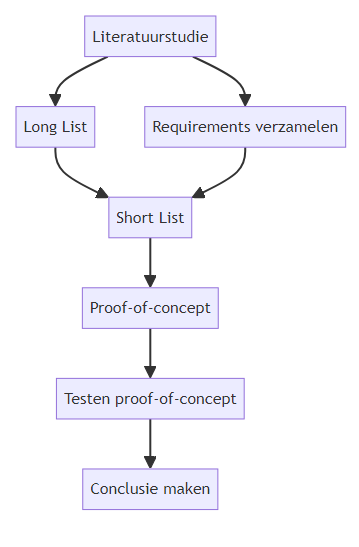
\includegraphics[width=.4\textwidth]{graphics/flowchart.png}
    \caption{\label{fig:flowchart}}Flowchart van methodologie
\end{figure}
%---------- Verwachte resultaten ----------------------------------------------
\section{Verwacht resultaat, conclusie}%
\label{sec:verwachte_resultaten}
Op basis van literatuuronderzoek zal gekozen worden om Bun te vergelijken met Node.js doordat dit framework zich focust op performantie.
De verwachte resultaten zijn metingen van de proof-of-concepts die aantonen dat Bun performanter is dan de Node.js (zie figuur~\ref{fig:uitvoeringstijd} en~\ref{fig:responstijd}). 
Deze metingen werden uitgevoerd met behulp van benchmark tools Hyperfine en Bombardier.
Ook wordt verwacht dat de package manager van Bun een snellere installatietijd heeft dan de Node Package Manager en dat Bun minder complex is dan Node.js (zie figuur~\ref{fig:installatietijd}).
Deze verwachtingen komen mede doordat Bun zich bij de ontwikkeling specifiek heeft gefocust op performantie-optimalisatie.
Ook heeft Bun redelijk wat zaken, zoals een test-runner, al ingebouwd wat het minder complex maakt dan Node.js.
Op basis van deze metingen kan een onderbouwde keuze worden gemaakt tussen het gebruik van Node.js en Bun bij de ontwikkeling
van performante webapplicaties.

Doordat Node.js nog altijd de norm is, zal het zeer veel tijd vragen tegen dat Bun deze effectief kan vervangen.
Het is toch belangrijk dat er nu een keuze kan gemaakt worden tussen javascript runtime-omgevingen bij de ontwikkeling van applicaties.

\begin{figure}
    \centering
    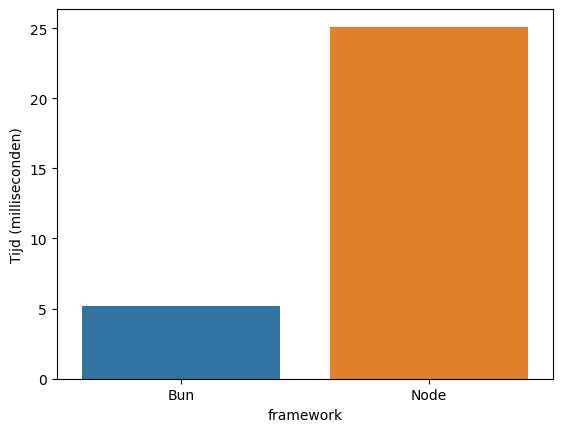
\includegraphics[width=.4\textwidth]{graphics/diagram.png}
    \caption{\label{fig:uitvoeringstijd}}Mock-up waarbij we zien dat Bun een betere uitvoeringstijd heeft dan Node.js bij de uitvoering van een simpel algoritme.
    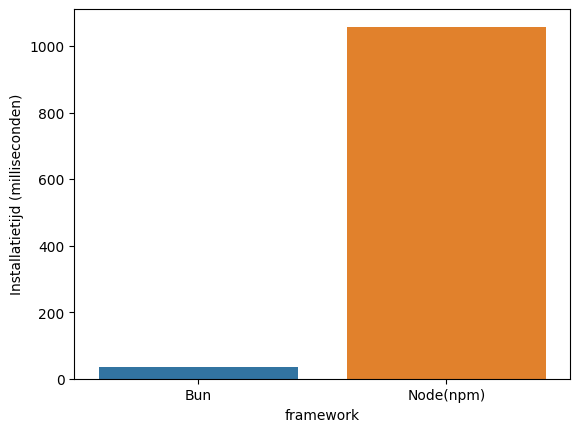
\includegraphics[width=.4\textwidth]{graphics/installatietijd.png}
    \caption{\label{fig:installatietijd}}Mock-up waarbij we zien dat Bun een betere installatietijd heeft dan Node.js bij het installeren van dependencies.
    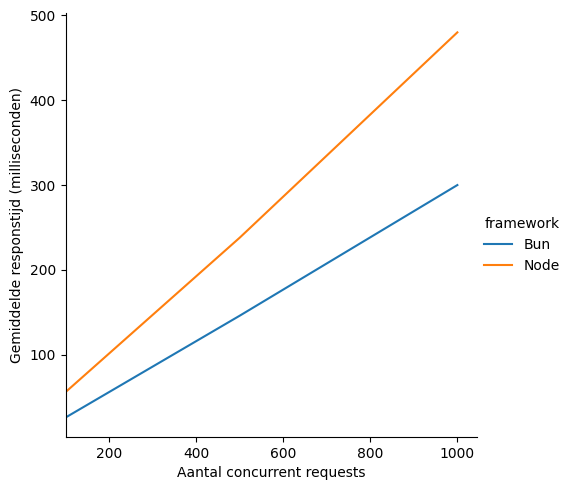
\includegraphics[width=.4\textwidth]{graphics/Responstijd.png}
    \caption{\label{fig:responstijd}}Mock-up waarbij we zien dat Bun een betere responstijd heeft dan Node.js bij het afhandelen van concurrent requests.
\end{figure}


%%---------- Andere bijlagen --------------------------------------------------
% TODO: Voeg hier eventuele andere bijlagen toe. Bv. als je deze BP voor de
% tweede keer indient, een overzicht van de verbeteringen t.o.v. het origineel.
%\input{...}

%%---------- Backmatter, referentielijst ---------------------------------------

\backmatter{}

\setlength\bibitemsep{2pt} %% Add Some space between the bibliograpy entries
\printbibliography[heading=bibintoc]

\end{document}
